\documentclass[tikz,border=5mm]{standalone}
\usepackage{pgfplots}
\usepackage{pgfplotstable}
\pgfplotsset{compat=1.17}

\begin{document}

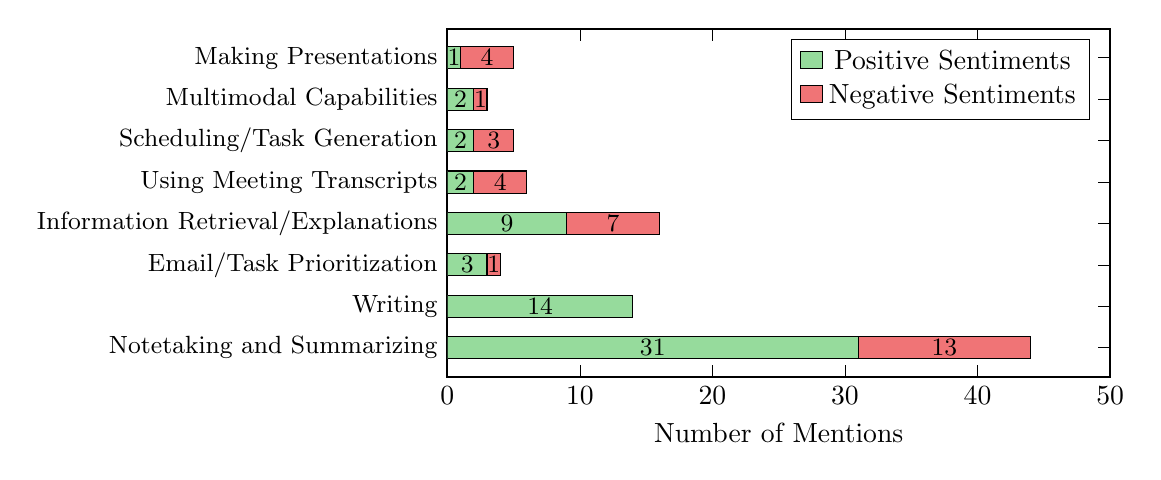
\begin{tikzpicture}[scale=1] % Reduce overall figure size
\definecolor{red}{RGB}{240,116,118}
\definecolor{green}{RGB}{150,219,156}

% Define the data inline (fixing column formatting)
\pgfplotstableread{
Label                                Positive  Negative
{Notetaking and Summarizing}          31       13
{Writing}                             14       0
{Email/Task Prioritization}           3       1
{Information Retrieval/Explanations}  9       7
{Using Meeting Transcripts}           2       4
{Scheduling/Task Generation}          2       3
{Multimodal Capabilities}             2       1
{Making Presentations}                1       4
}\sentimentdata

\begin{axis}[
    xbar stacked,   
    xmin=0, xmax=50, 
    width=10cm, height=6cm, % Adjust figure size
    xlabel={Number of Mentions},
    ytick=data,    
    yticklabels from table={\sentimentdata}{Label},  
    bar width=8pt,
    enlarge y limits=0.1,
    legend pos=north east, % Move legend inside plot area
    nodes near coords,
    every node near coord/.append style={font=\small}, 
    axis line style={draw=black, thick},
    tick style={draw=black},
    yticklabel style={align=right, font=\small} 
]

% Add the bars
\addplot [fill=green] table [x=Positive, meta=Label, y expr=\coordindex] {\sentimentdata};  
\addplot [fill=red] table [x=Negative, meta=Label, y expr=\coordindex] {\sentimentdata};  

\legend{Positive Sentiments, Negative Sentiments}

\end{axis}

\end{tikzpicture}

\end{document}
